\documentclass{aa}
\usepackage{graphicx,txfonts}
\usepackage[hidelinks]{hyperref}
\journalname{Euclid Deep Field North}
\makeatletter
\renewcommand*\aa@manuscriptname{\quad\textnormal{Research report}}
\renewcommand*\aa@textidlineempty{\textit{Euclid Deep Field North}}
\AtBeginDocument{%
  \renewcommand*\aa@numarticle{}%
  \renewcommand*\aa@pageof{Page \thepage}%
}
\makeatother
\hypersetup{pdfauthor={Biswajit Jana}}
% The A&A class enables review line numbering at the end of the document.
% These are reader-facing research reports.
\renewcommand{\linenumbers}{\nolinenumbers}

\graphicspath{{../2026-11-14-day01/analysis/real_results/}}
\begin{document}
\hypersetup{pdftitle={H-alpha flux and photometric aperture radius in Euclid Deep Field North}}
\title{H$\alpha$ flux and photometric aperture radius in Euclid Deep Field North}
\subtitle{Day 1. A single-tile morphology pilot}
\author{Biswajit Jana}
\institute{Independent researcher, United Kingdom}
\date{14 November 2026}
\abstract
{Euclid VIS imaging and NISP spectroscopy allow H$\alpha$-selected galaxies to be compared by observed optical aperture size.}
{We test whether fitted H$\alpha$ flux and MER Kron aperture radius are associated at comparable catalogue redshift and VIS brightness.}
{We select a $0.15^{\circ}$ cone from Euclid DR1-Foundation. We combine eligible H$\alpha$ fits by object and compare high- and low-flux halves in redshift and VIS-flux strata. Original morphology measurements are available for one of the five contributing tiles.}
{Of 426 selected objects, 327 have a morphology match and 150 pass all imaging cuts. Before those cuts the aperture contrast is $+0.04856$ dex. Median Kron radii are 26.22 and 28.34 pixels for the retained and excluded matches, respectively.}
{Incomplete morphology coverage and imaging selection change the sample. The 150 retained objects fall below the predeclared minimum of 200.}
\keywords{galaxies: photometry -- galaxies: statistics -- methods: observational -- techniques: imaging spectroscopy}
\maketitle
\section{Introduction}
Euclid DR1-Foundation provides matched optical imaging and slitless spectra in Euclid Deep Field North \citep{aussel2026}. The MER Kron radius is the semi-major axis of the detection-image aperture. Its value in pixels responds to the light profile, angular resolution and blending. PSF-corrected galaxy shape inference and spatially resolved NISP line maps address different observables \citep{dunn2026,gabarra2026}. Here the question is whether the released H$\alpha$ flux is associated with the observed aperture radius within a line-selected pilot sample.

\section{Observations and methods}
The cone is centred at ICRS RA $269.733^{\circ}$ and Dec $+66.018^{\circ}$. It contains 55\,123 MER records and 22\,665 rank-0 H$\alpha$ rows. Of the latter, 15\,942 carry an invalid-flux sentinel. Positive flux and uncertainty with S/N~$\geq5$ leave 3121 fits for 1522 distinct objects. The redshift cut $0.90\leq z\leq1.50$ retains 663. Requiring redshift probability $\geq0.99$, a VIS detection and positive VIS aperture flux retains 426 objects. The object-level line flux is the median of eligible fits, some of which share exposures.

The morphology join uses exact object IDs and original MER FITS tile 101834044. The full imaging cuts require positive Kron radius, zero VIS and detection-quality flags, and spurious probability below 0.5. The comparison uses redshift bins $[0.90,1.10)$, $[1.10,1.30)$ and $[1.30,1.50)$ with VIS-flux tertiles in each bin. Cells require at least 20 objects, including at least ten per H$\alpha$ half. The estimator is
\begin{equation}
\Delta=\frac{\sum_j n_j\left[\widetilde{\log_{10}r}_{j,\mathrm{hi}}-\widetilde{\log_{10}r}_{j,\mathrm{lo}}\right]}{\sum_j n_j},
\end{equation}
where the tildes denote medians within cell $j$ and $r$ is the MER aperture radius. The exploratory bootstrap resamples within H$\alpha$ halves. The original $1.25^{\circ}$ test requires 200 clean objects and four eligible cells.

\begin{figure*}[t]
\centering
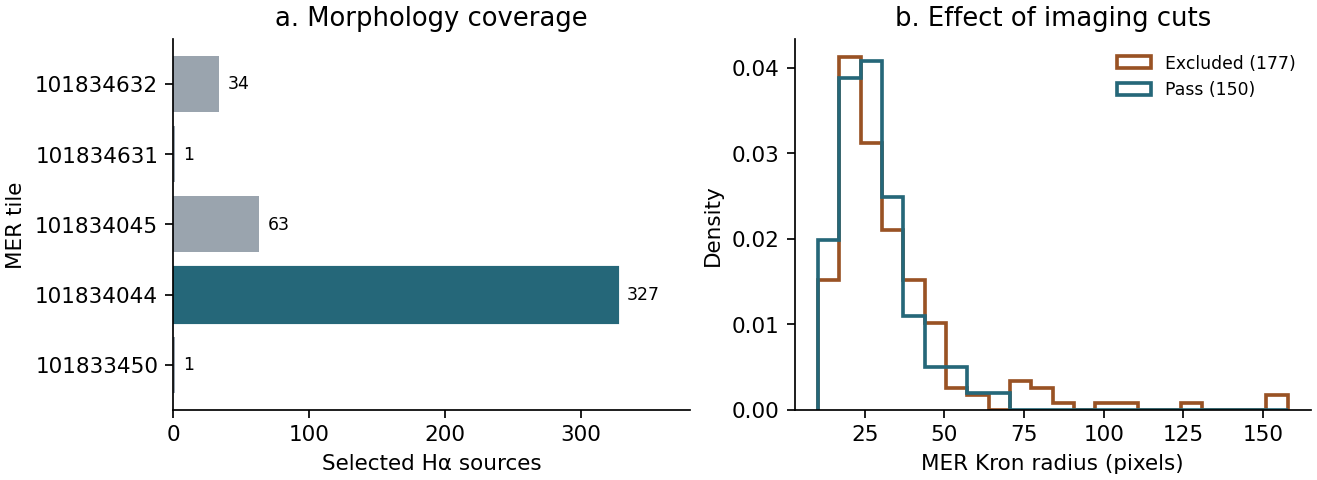
\includegraphics[width=.61\textwidth]{selection_diagnostics.png}
\caption{Morphology coverage and imaging selection. The highlighted tile supplies all 327 original morphology matches. The right panel compares the Kron radius distributions of the 150 retained and 177 excluded matches.}
\label{fig:selection}
\end{figure*}

\section{Results}
The selected objects span five tiles (Fig.~\ref{fig:selection}). The 99 objects without a retrieved morphology measurement represent 23.2\% of the selected sample. Their median VIS aperture flux is 1.062~$\mu$Jy, compared with 0.967~$\mu$Jy for the matched sources. Within the matched sample, 155 objects have nonzero VIS flags and 177 have nonzero detection-quality flags. These counts overlap. No source fails the spurious-probability cut.

Before the final imaging cuts, nine cells give $\Delta=+0.04856$ dex with exploratory 95\% bootstrap endpoints $+0.00693$ and $+0.09182$ dex. The point estimate corresponds to an 11.8\% aperture-radius ratio difference. Two archived implementations give nominal permutation $p$ values of 0.01249 and 0.02249. The estimates describe the pre-cut sample. Within the 426 selected emitters, H$\alpha$ and VIS flux have Spearman $\rho=0.452$ (95\% bootstrap interval 0.362--0.536).

\begin{figure}[t]
\centering
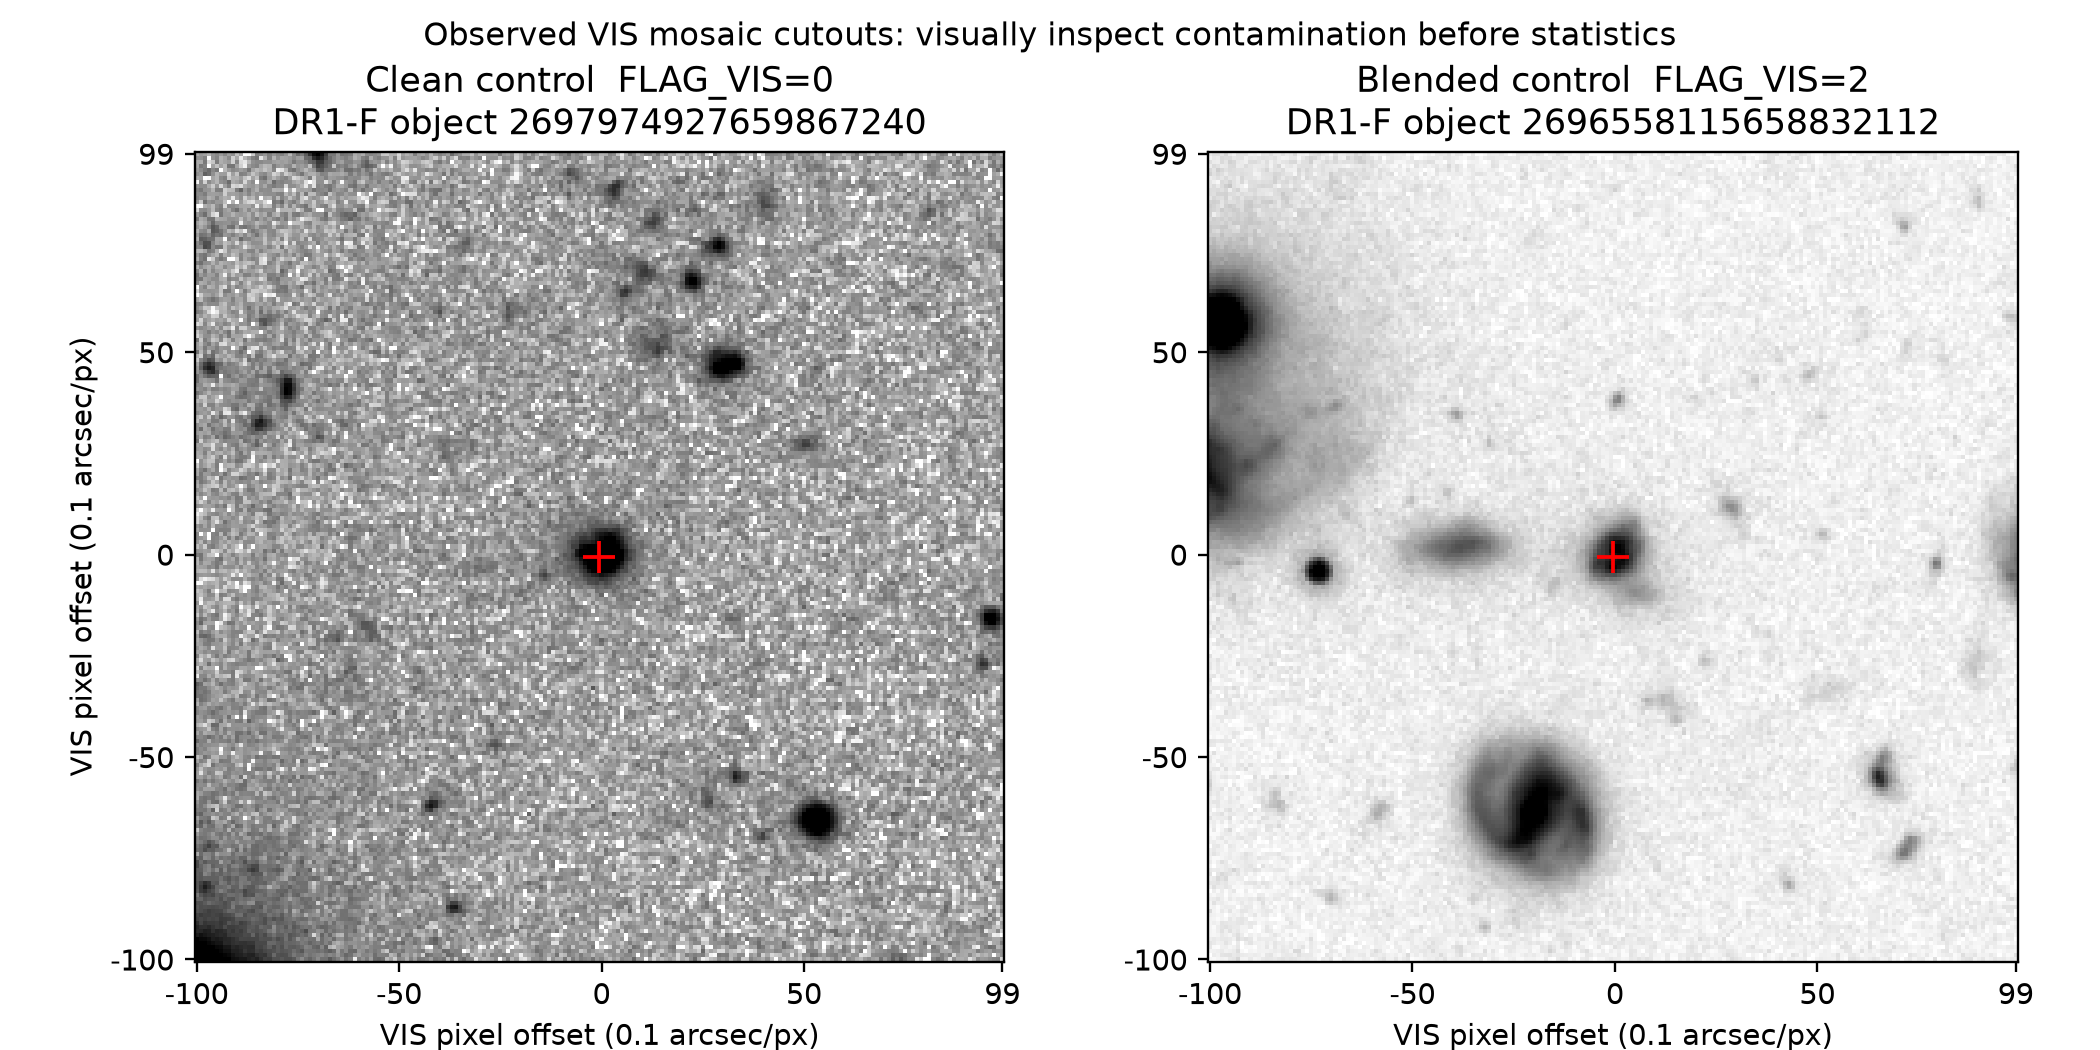
\includegraphics[width=\columnwidth]{figures/euclid_vis_clean_vs_blended_real.png}
\caption{VIS cutouts of the clean (left) and blended (right) catalogue examples. The target lies at the central marker.}
\label{fig:flags}
\end{figure}

\section{Discussion and conclusions}
The blended example in Fig.~\ref{fig:flags} shows neighbouring structure. The retained sample has a 7.5\% smaller median Kron aperture and a 13.8\% lower median H$\alpha$ flux than the excluded matches. Median redshifts are 1.142 and 1.145, respectively. Imaging selection therefore changes the aperture and line-flux distributions even when the redshift medians are similar. A separate NISP masking example has 190 of 433 bins passing the mask and quality threshold across 8548.5--13\,862.1~\AA. This example illustrates coverage. The Day 2 spectra are matched directly to the selected objects.

The 150 retained sources fall below the predeclared minimum of 200. An inference about intrinsic galaxy sizes requires PSF-corrected measurements and a model of the H$\alpha$ selection function. The original $1.25^{\circ}$ field remains untested.

\section*{Data availability}
The \href{https://github.com/Biswajit1999/daily-astro-notebooks/tree/master/euclid-dr1-foundation/2026-11-14-day01}{repository} supplies the archive extracts, figures, and Python scripts. IRSA DOIs are \href{https://doi.org/10.26131/IRSA675}{10.26131/IRSA675} (MER), \href{https://doi.org/10.26131/IRSA696}{10.26131/IRSA696} (SPE redshifts), and \href{https://doi.org/10.26131/IRSA692}{10.26131/IRSA692} (SPE lines).
\begin{acknowledgements}
This work has made use of the Data Release (DR1) data from the Euclid mission of the European Space Agency (ESA), distributed by NASA/IPAC IRSA.
\end{acknowledgements}
\bibliographystyle{aa}
\bibliography{references}
\end{document}
